\documentclass[../entwurf.tex]{subfiles}

\begin{document}
\section{Sequenzdiagramme}
\subsection{Starten eines Songs aus der Audiobibliothek}
\begin{center}
	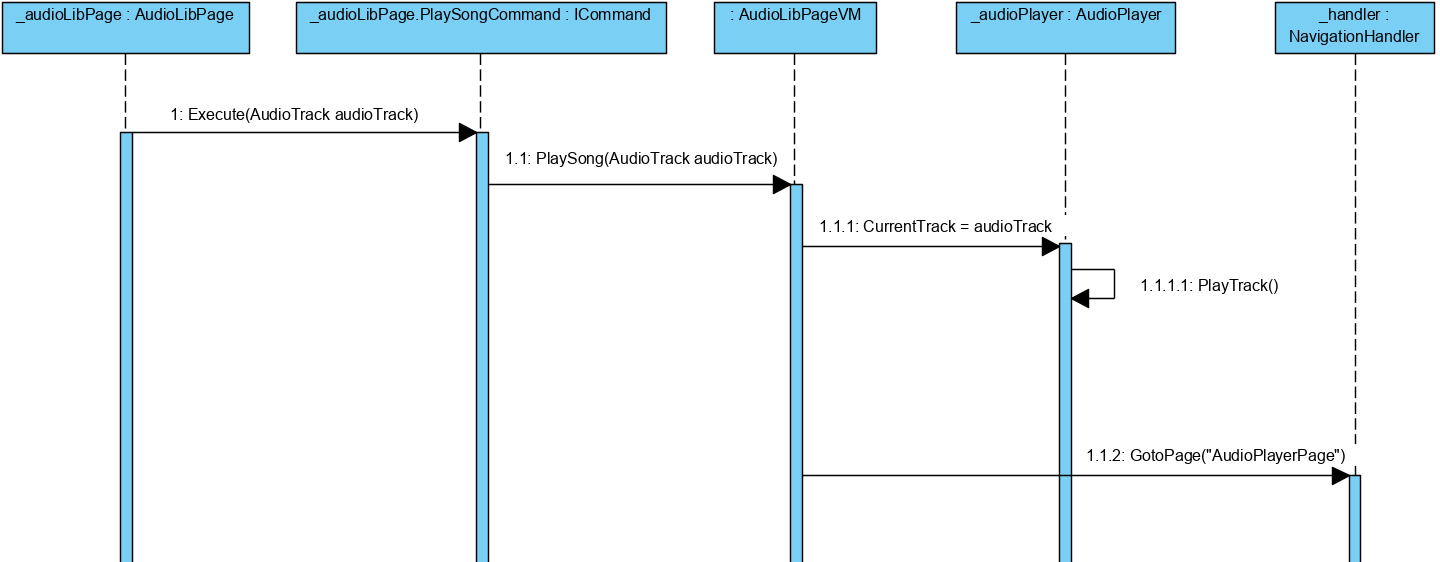
\includegraphics[page=1,width=350pt,keepaspectratio]{../graphics/sequenz_diagramme/PlaySongSequenzDia.png}
\end{center}
Das Sequenz-Diagramm stellt dar was passiert, nachdem der User auf einen Song in der AudioLibrary gedrückt hat.
\paragraph{Beschreibung}
Die View-Klasse \code{AudioLibPage} führt (unter Anwendung von \Gls{databinding}) einen dafür vorgesehenen \code{ICommand} aus dem ViewModel aus (\code{execute()}).
Dies führt zu einem Ausführen von \code{PlaySong(AudioTrack audioTrack)} in der \code{AudioLibPageVM},
was dazu führt,dass in der Klasse AudioTrack der \code{CurrentTrack} auf \code{audioTrack} gesetzt wird   und die Methode \code{playTrack()} in der Model-Klasse \code{AudioPlayer} aufgerufen wird. Danach wird durch den Aufruf von \code{GotoPage(''AudioPlayerPage'')} im \code{NavigationHandler} zur \code{AudioPlayerPage} gewechselt.

\subsection{Suchen neuer ESense Earables}
Das folgende Sequenz-Diagramm stellt dar was passiert, wenn der User auf der ConnectionPage auf den Refresh-Button drückt.
\begin{center}
	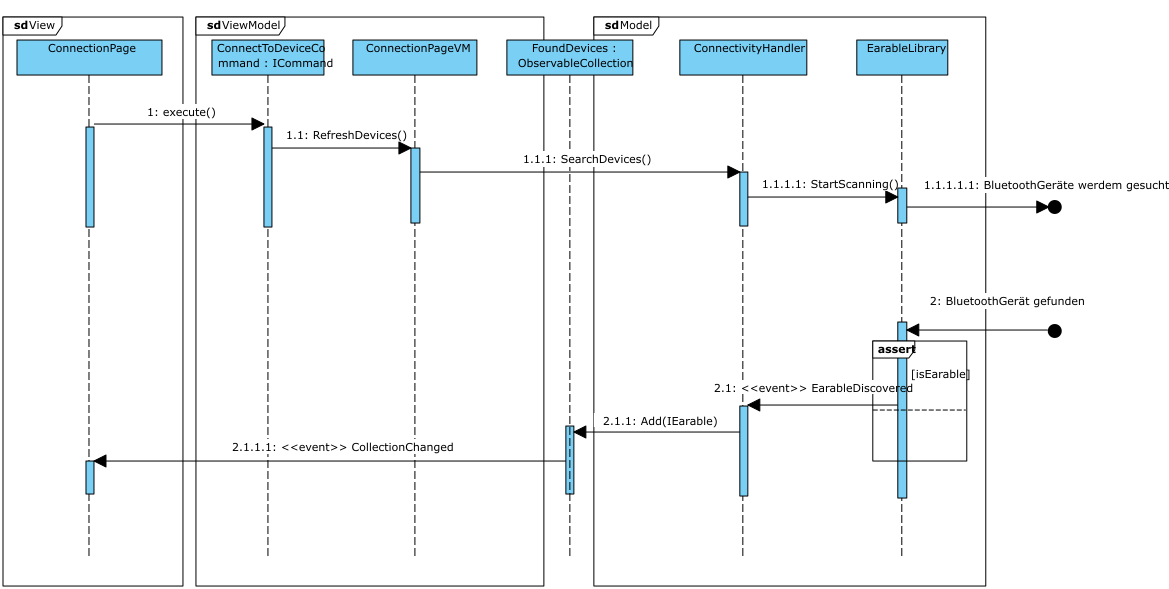
\includegraphics[page=1,width=350pt,keepaspectratio]{../graphics/sequenz_diagramme/RefreshFoundDevices.png}
\end{center}
\paragraph{Beschreibung}
Die View-Klasse \code{ConnectionPage} führt (unter Anwendung von \Gls{databinding}) einen dafür vorgesehenen \code{ICommand} aus dem ViewModel aus (\code{execute()}).
Dies führt zu einem Ausführen von \code{RefreshDevices()} in der \code{ConnectionsPageVM},
was wiederum einen Aufruf von \code{SearchDevices()} in der Model-Klasse \code{ConnectivityHandler} induziert.
Dies wiederum startet den Suchvorgang in der \code{EarableLibrary} (\code{StartScanning()}).
Im weiteren führt das Betriebssystem eine Suche nach Bluetooth-Geräten aus.
Für jedes derart gefundenes Gerät überprüft die \code{EarableLibrary} zunächst, ob es sich dabei um ein Earable-Gerät handelt.
Ist dem so, wird mittels \Gls{event} (\code{EarableDiscovered}) der \code{ConnectvitiyHandler} aufgerufen.
Dieser verwaltet eine interne Liste (\code{FoundDevices}), welche alle aktuell in der Nähe befindlichen Earables auflistet.
Da es sich hierbei um eine \code{ObservableCollection} handelt - welche durch eine weitergeleitete \Gls{property} im ViewModel auch der View zur Verfügung steht -
kann diese durch ein weiteres \Gls{event} (\code{CollectionChanged}) über die Änderung informiert werden und das neue Gerät anzeigen.

\subsection{Aktivieren eines Modus}
\begin{center}
	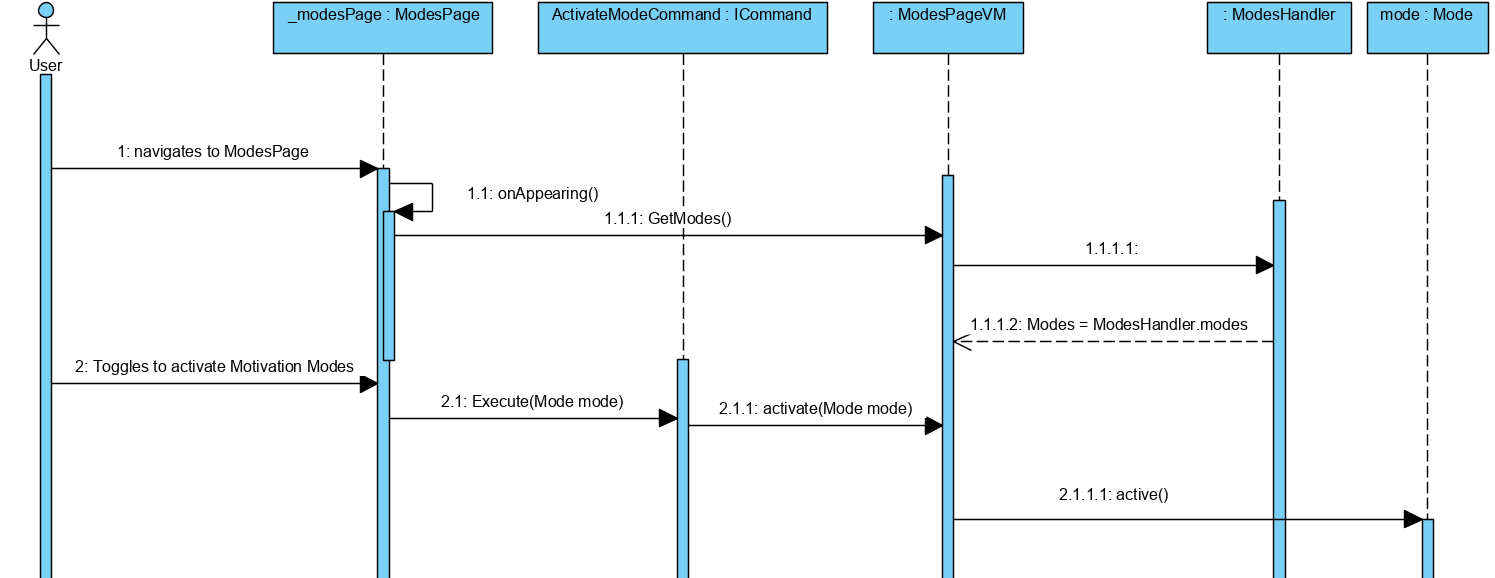
\includegraphics[page=1,width=350pt,keepaspectratio]{../graphics/sequenz_diagramme/ActivateModeDia.png}
\end{center}
Das Diagramm stellt dar was passiert, wenn der User auf die ModePage wechselt und dann einen beliebigen Modus der App aktiviert.
\paragraph{Beschreibung}
Nachdem der User auf die \code{ModesPage} gewechselt hat, wird im Code-Behind der Klasse  \code{onAppearing()} aufgerufen. Innerhalb der Methode im zugehörigen ViewModel wird \code{GetModes()} aufgerufen, wodurch aus der Model-Klasse \code{ModesHandler} die aktuell verfügbaren Modi in Form von Objekten der Klasse \code{Mode} geladen werden und in der Variable \code{Modes} gespeichert werden.

Wenn der User dann durch toggeln eines Switchs den zugehörigen Modus aktiviert, wird (unter Anwendung von \Gls{databinding}) ein dafür vorgesehener \code{ICommand} aus dem ViewModel ausgeführt(\code{execute()}). Dies führt dazu, dass \code{activate(Mode mode)} in der \code{ModesPageVM} ausgerufen wird. In der \code{ModesPageVM} wird danach \code{activate()} auf dem übergebenen \code{Mode mode} ausgeführt.

\subsection{Verwendung des AutoStop Modus}
\begin{center}
	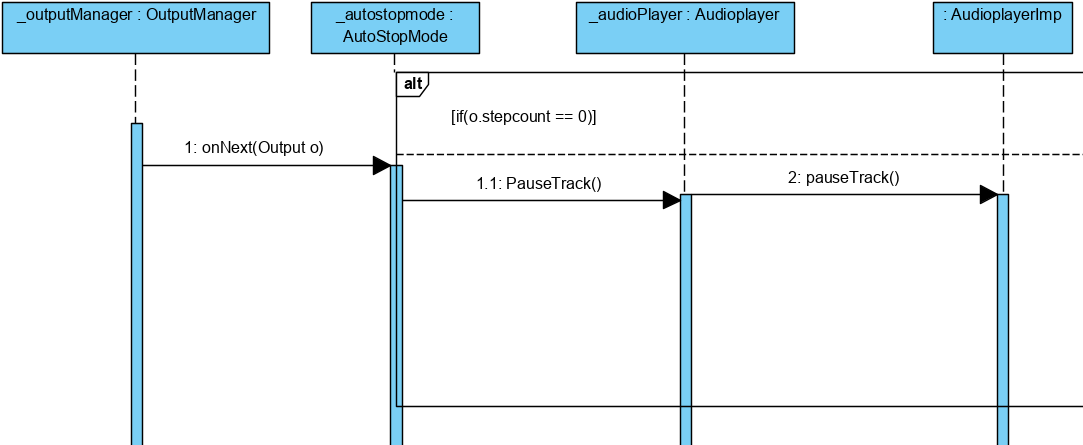
\includegraphics[page=1,width=350pt,keepaspectratio]{../graphics/sequenz_diagramme/AutoStopDia.png}
\end{center}
Das Sequenz-Diagramm stellt dar was passiert wenn der User bei gestartetem AutoStop-Modus das Laufen unterbricht und stehen bleibt.
\paragraph{Beschreibung}
Solange die App aktiv Schritte erkennt(wenn ein paar ESense Earables verbunden sind) wird mit der Methode \code{onNext()} durch ein Objekt der Klasse \code{Output} die Schrittanzahl innerhalb eines festgelegten Zeitraum übergeben. Fällt die Anzahl der Schritte innerhalb des festgelegten Zeitraums auf 0, wird bei aktiviertem AutoStop-Modus durch den \code{AutoStopMode \_autoStopMode}  \code{PauseTrack()} auf 
dem Objekt \code{AudioPlayer \_audioPlayer} ausgerufen. Dieser ruft dann auf einer Implementierung eines Audioplayers \code{PauseTrack()} auf.
\end{document}
